%This is the first chapter of the dissertation

%The following command starts your chapter. If you want different titles used in your ToC and at the top of
%the page throughout the chapter, you can specify those values here. Since Columbia doesn't want extra
%information in the headers and footers, the "Top of Page Title" value won't actually appear.

%By using the asterisk to start a new section, I keep the section from appearing in the table of contents.
%If you want your sections to be numbered and to appear in the table of contents, remove the asterisk.



\pagestyle{cu}
\graphicspath{{./Chapter1/Figures/}}
\chapter[Dark Matter][Dark Matter]{Dark Matter}
\label{chap:dark_matter}

For much of the last century evidence has been building for two non-luminous components of our universe that cannot be explained with
our current model of physics.  The first is the acceleration of the expansion of the universe, which is hypothesized to result from an
unknown kind of energy known as dark energy.  Measurements estimate dark energy composes ${\sim}70$\% of
matter in the current observable universe.  The second is the presence of a gravitational field that is many times too large to be caused
by ordinary - or baryonic - matter, but whose source cannot be seen.  Dark matter (DM) is a hypothetical form of matter that does not
interact electromagnetically and provides the additional massive component that would solve this discrepancy.  Observations predict that
dark matter
constitutes ${\sim}26$\% of the universe.  In dark energy and dark matter the term ``dark'' is a relic from their early histories and
today both are understood to be invisible.

This chapter presents an overview of dark matter and the different methods of detection.  It begins with a summary of the
$\Lambda \mathrm{CDM}$ model (\secref{sec:dark_matter_lambda_cdm}) followed by a discussion on evidence of dark matter's existence
(\secref{sec:dark_matter_evidence}) and potential DM candidates (\secref{sec:dmcandidates}).  Next detection methods for Weakly
Interacting Massive Particle (WIMP) dark matter are detailed (\secref{sec:detection}), and the final section covers the various
categories of direct detection experiments (\secref{sec:direct_detect}).



%====================================
\section[$\Lambda$CDM Model][$\Lambda$ CDM Model]{$\boldsymbol{\Lambda}$CDM Model}
\label{sec:dark_matter_lambda_cdm}
The $\Lambda \mathrm{CDM}$ model describes the evolution of the universe from its inception at the Big Bang to present day.  It is named
from its inclusion of a cosmological constant (dark energy) $\Lambda$ and cold dark matter (CDM) (\secref{subsec:hot_vs_cold}), and is the
most successful model to
date.  $\Lambda$ is understood to be an energy density that is uniform throughout the observable universe and interacts repulsively with
itself to drive the universe's expansion.  Cold dark matter is predicted to be a non-relativistic, non-luminous form of matter that
interacts primarily through gravitation.  The validity of the $\Lambda \mathrm{CDM}$ model is dependent on our universe being homogeneous
and isotropic over large
(${\sim} 100\ \mathrm{Megaparsecs}$ - Mpc) distances,
Einstein's General Relativity, and a path connected universe - all of which are believed to be true.  Under these assumptions Einstein's
field equations can be solved for the Friedmann-Lema\^{i}tre-Robertson-Walker (FLRW) metric, which in polar coordinates is

\begin{equation}
ds^{2} = -c^{2}dt^{2} + a(t)^{2} \bigg( \frac{dr^{2}}{1 - kr^{2}} + r^{2}d\Omega^{2} \bigg)
\label{eq:dark_matter_lambda_cdm_rw_metric}
\end{equation}

\noindent where $ds$ is the distance traversed in space-time, $c$ is the speed of light, $t$ is time, and $r$ and
$d\Omega = d\theta^2 + \mathrm{sin}^2(\theta)d\phi^2$ are spatial coordinates.  $a(t)$ is known as the scale factor with $a=1$ today, and
$k \in \{-1, 0, 1\}$ is the curvature of the
universe.  A universe with $k = -1$ is an open universe and has negative curvature.  Its geometry is hyperbolic, meaning the
sum of the angles in a triangle is $< 180^{\circ}$ and two lines that do not cross are never equidistant.  An open universe will expand
forever as long as $\Lambda \geq 0$ (observations disqualify a universe with negative $\Lambda$).  A universe with $k = 0$ is flat and
has Euclidean geometry (angles in a triangle equal $180^{\circ}$ and parallel lines remain equidistant).  If $\Lambda = 0$ it will
expand forever at a decelerating rate, asymptotically approaching 0.  For $\Lambda > 0$ the expansion first slows due to gravity but will
ultimately increase as the average density of the universe $\rho$ decreases.  A universe with $k = 1$ is closed and has positive
curvature.  Its geometry is similar to a sphere: the angles in
a triangle sum to ${>}\, 180^{\circ}$ and all lines eventually meet.  The fate of a closed universe depends on the fraction of its
components.  If $\Lambda = 0$ the expansion will come to a stop and begin to
contract, returning to a singularity known as the ``Big Crunch''.  However, if enough dark energy is present the universe will follow
an open or flat universe and expand forever.  As the density of gravitationally-interacting components increases a larger $\Lambda$ is
necessary to prevent a Big Crunch.

Einstein's field equations for the solution in \eqnref{eq:dark_matter_lambda_cdm_rw_metric} give the Friedmann Equations

\begin{equation}
\bigg(\frac{\dot{a}}{a}\bigg)^{2} = \frac{8\pi G \rho}{3} - \frac{k}{a^{2}}
\label{eq:friedman1}
\end{equation}

\begin{equation}
\frac{\ddot{a}}{a} = -\frac{4\pi G}{3}(\rho + 3p)
\label{eq:friedman2}
\end{equation}

\noindent where $\dot{a}/a$ is referred to as the Hubble
constant $H$ ($H = H_{0}$ today) and $p$ is the pressure.  The density for a flat universe, known as the critical density, can be derived
from \eqnref{eq:friedman1} to be $\rho_{\mathrm{crit}} = 3H^2 / 8\pi G$.  A useful
notation is the ratio of the density to the critical density, known as the density parameter,
$\Omega := \rho/\rho_{\mathrm{crit}}$.  Moving forward $\Omega$ will represent the density
parameter rather than spatial coordinates as in \eqnref{eq:dark_matter_lambda_cdm_rw_metric}.  Substituting
$\Omega$ into \eqnref{eq:friedman1} gives

\begin{equation}
\Omega - 1 = \frac{k}{H^{2}{a^{2}}}
\label{eq:dark_matter_lambda_cdm_dens_par}
\end{equation}

\eqnref{eq:dark_matter_lambda_cdm_dens_par} shows that the universe will be open for $\Omega < 1$, flat for $\Omega = 1$, and
closed for $\Omega > 1$.  The density parameter can be decomposed as $\Omega = \sum \Omega_{i}$ where $\Omega_{i}$ is a component of the
universe.  Measurements estimate density parameters of $\Omega_{\mathrm{b}} \sim 0.05$ for baryonic matter,
$\Omega_{\mathrm{dm}} \sim 0.26$ for non-baryonic (dark)
matter, $\Omega_{\mathrm{r}} \sim 0$
for radiation, and $\Omega_{\Lambda} \sim 0.69$ for dark energy (\secref{subsec:cmb}).  These numbers reveal cold dark matter and dark
energy are the dominant components, making up $> 94\%$ of the total matter density.



%====================================
\section[Evidence for Dark Matter][Evidence for Dark Matter]{Evidence for Dark Matter}
\label{sec:dark_matter_evidence}
%========
\subsection{Dynamical Contraints} \label{subsec:dynamics}
The first evidence for Dark Matter appeared in 1933 when Swiss astronomer Fritz Zwicky was observing the Coma Cluster
and noticed the velocity of the galaxies was too large to be explained by the luminous matter.  He argued that if there were
some additional mass that only acted gravitationally it could explain his observations, and estimated it
to be approximately $400$ times greater than the visible matter \citeref{Zwicky1933}.  Today this factor is much
smaller as advances in technology have shown the luminous matter is larger, but the discrepancy persists.  Zwicky coined this mystery
matter \textit{dunkel Materie} or ``dark matter".  Since then other galaxy clusters have been observed and support this claim.

In 1970 Vera Rubin and Kent Ford used H$\alpha$ from H II regions to measure the rotation of stars around the
center of the Andromeda galaxy \citeref{Rubin1970}.  The virial theorem predicts $v(r) = \sqrt{GM(r)/r}$ so
that at large radii the velocity of the galaxies should decrease as $r^{-1/2}$.  Rubin and Ford's observations
contradicted the $M(r)$ derived from luminous mass.  As with Zwicky's measurement, the results could be
explained by introducing a non-luminous feature - in this case one with $M(r) \sim r$.  Observations of more than
one hundred thousand galaxies have since shown similar results, with DM halos containing several times the
luminous mass.

One example is galaxy NGC 6501.  The dark halo mass density in \figref{fig:ngc_6501} is estimated as
$\rho (r) = \rho_{0} \Big[ 1 + \Big( \frac{r}{r_{c}} \Big)^{2} \Big]^{-1}$ where $\rho_{0}$ and $r_{c}$
are the central halo mass density and radius, respectively, by fitting a least square to the velocity
distribution \citeref{Begeman1991}.  The left panel shows the mass of luminous matter decreases after
peaking at roughly $2\ \mathrm{kiloparsecs\ (kpc)}$, but the DM increases and at $>10$ kpc is proportional to $r$, causing
the rotational velocity to flatten.  Unfortunately, substantiated models that predict the
masses of a galaxy's disk, bulge, and halo independently do not exist, which makes dissociating the mass of baryonic matter from
DM difficult.  Most models expect the luminous matter to compose the galaxy's disk and bulge while the dark matter forms
the halo \citeref{Sofu2001}.



\begin{figure}
\centering
\captionsetup[subfigure]{labelformat=empty}
\ffigbox[\linewidth]{%
  \begin{subfloatrow}
\ffigbox[\FBwidth][]{\caption{}}{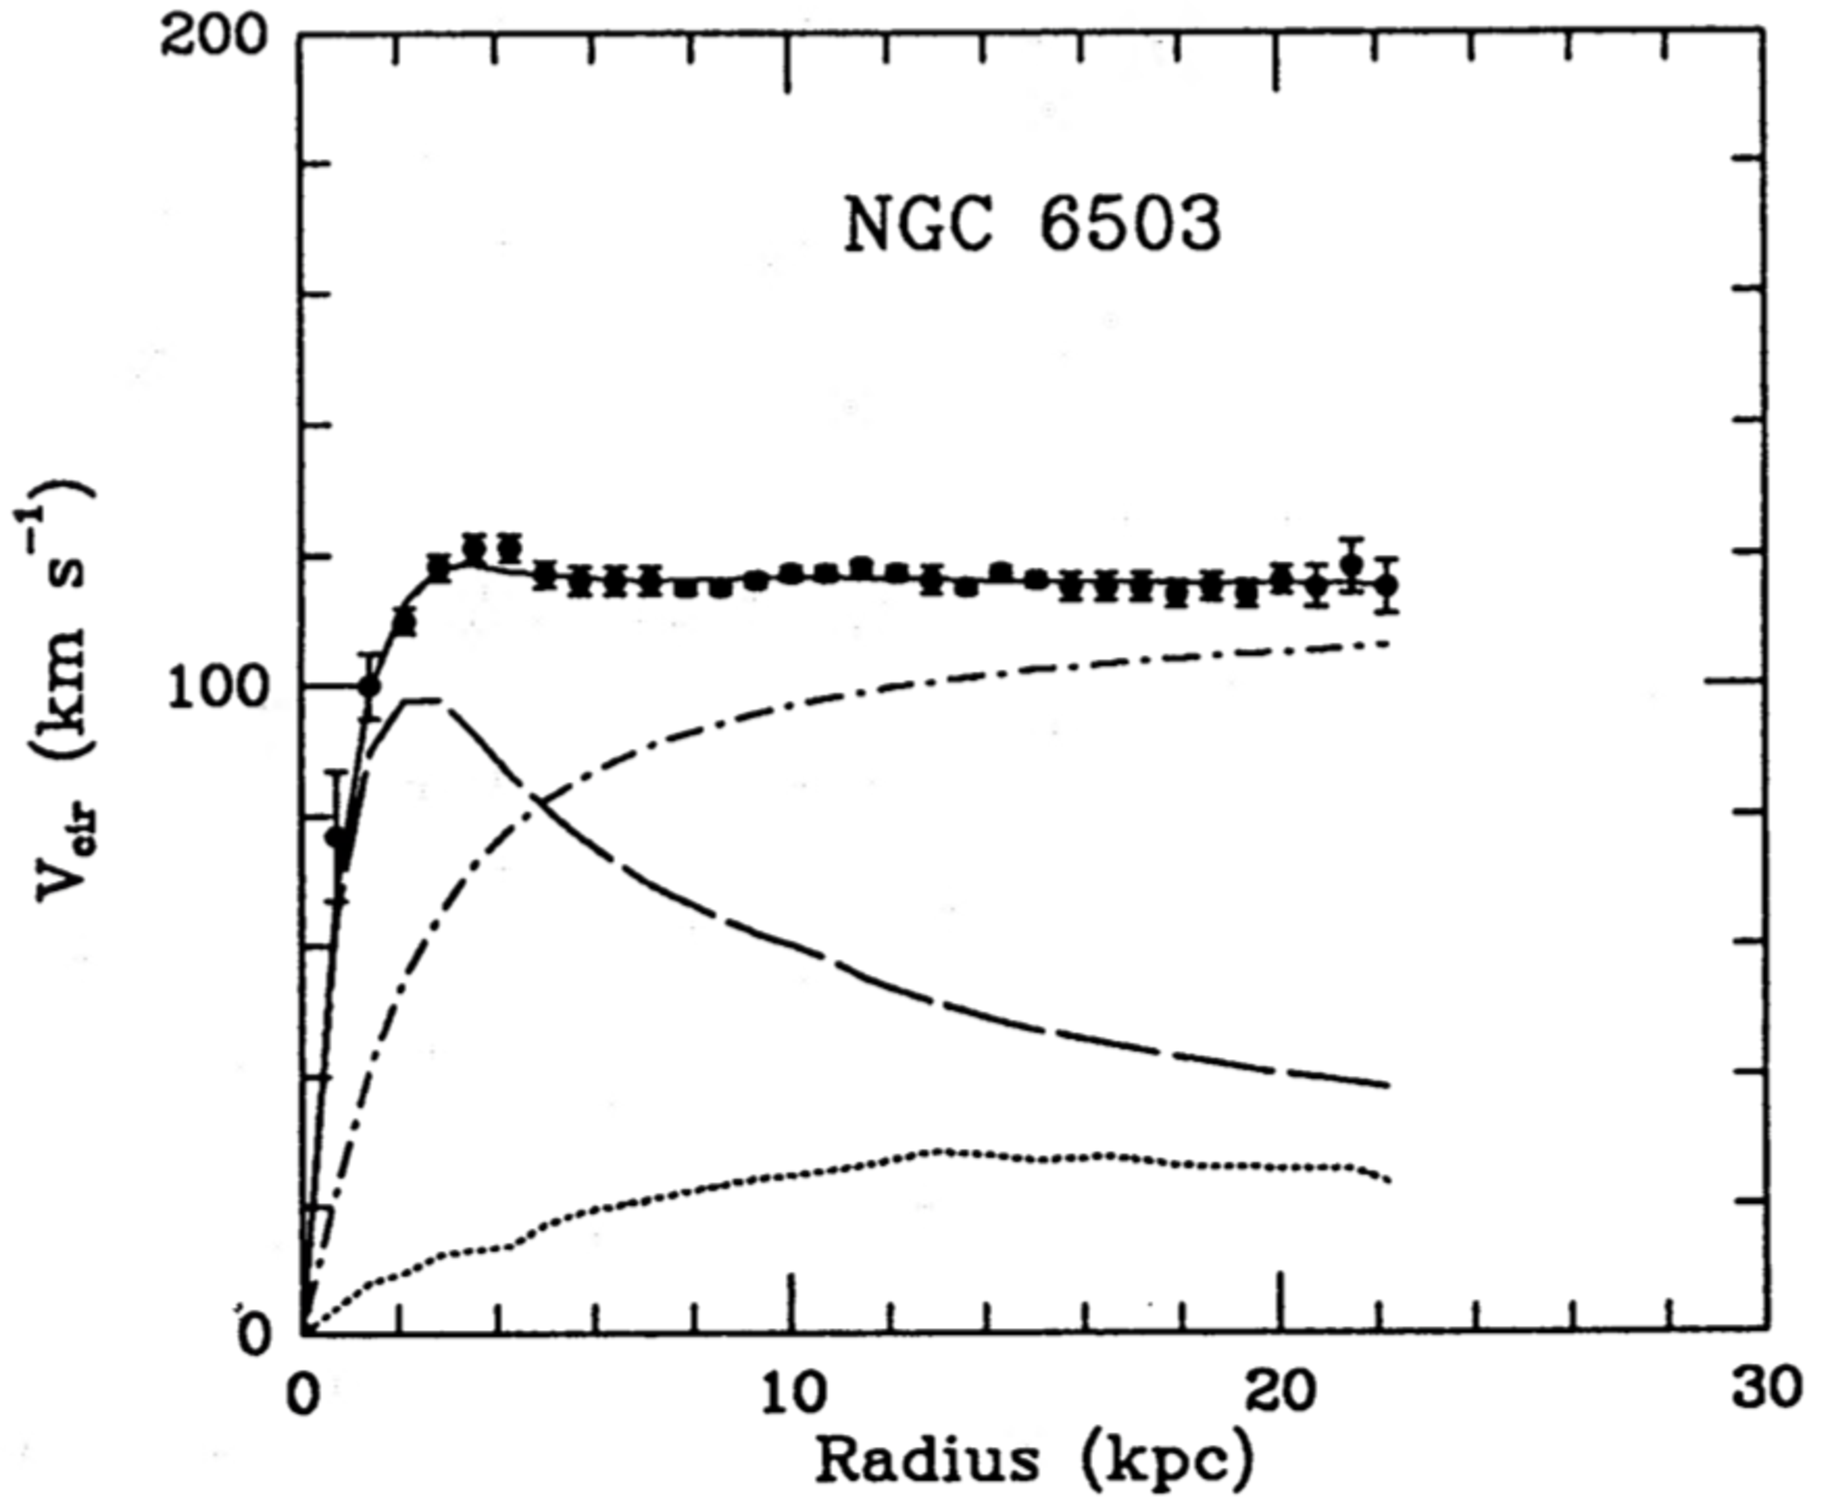
\includegraphics[height=5cm]{ngc_6503}}
  \end{subfloatrow}
  \hspace*{\columnsep}
  \begin{subfloatrow}
\vbox to 5.3cm{
  \ffigbox[\FBwidth]{\caption{}}
  {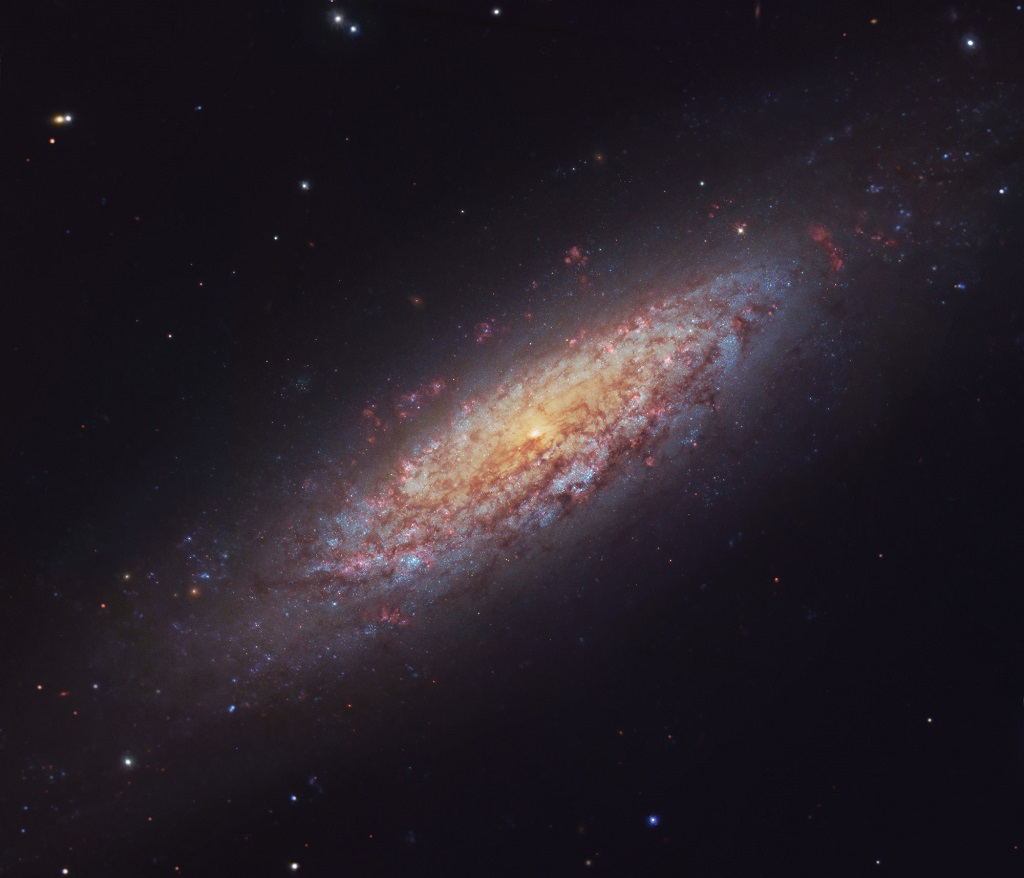
\includegraphics[trim={2cm, 2cm, 2cm, 2cm}, clip, height=4.4cm]{ngc_6503_image}}
}
  \end{subfloatrow}
  }{
  \vspace*{-10mm}
  \caption[Rotational velocity vs. radius (left) and image (right) of galaxy NGC 6503.]{Rotational velocity vs. radius (left) and image
  (right) of galaxy NGC 6503.  In the left panel visible components are
  represented by the dashed line, gas by the dotted, and dark halo by the dashed-dotted.
Image credit: (left) \citeref{Begeman1991}, (right) \citeref{Gendler2018}.}
	\label{fig:ngc_6501}
  }
\end{figure}

%for figure trim info
%https://tex.stackexchange.com/questions/57418/crop-an-inserted-image





\begin{figure}
	\centering
	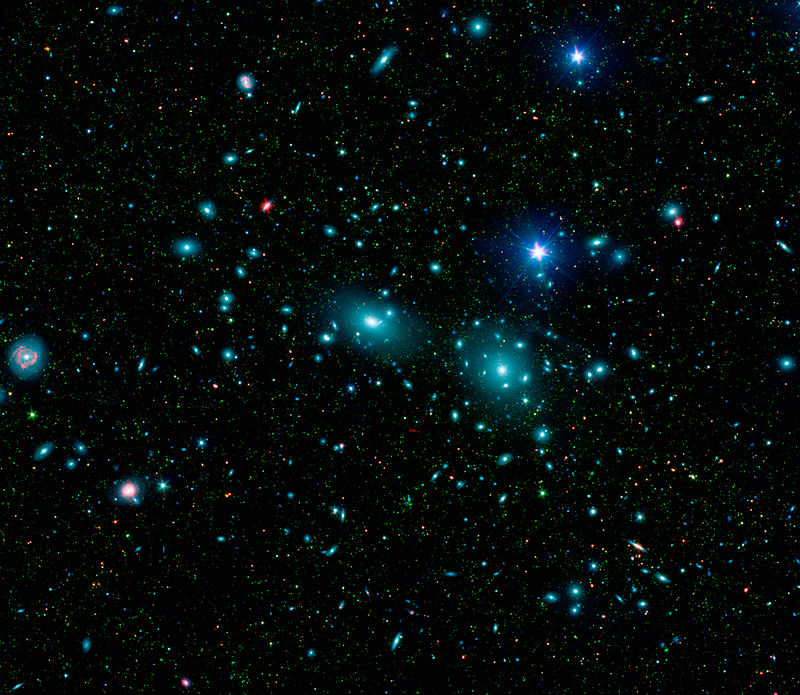
\includegraphics[width=0.5\textwidth]{coma_cluster}
	\label{fig:coma_cluster}
	\caption{Coma Cluster as seen by Sloan Digital Sky Survey and Spitzer Space Telescope.  Image credit: \citeref{NASA2018}.}
\end{figure}


%========

%========
\subsection{Gravitational Lensing}
\label{subsec:gravitational_lensing}
A collection of matter capable of bending electromagnetic radiation between a source and an observer is a gravitational
lens.  The deflection is caused by the matter's gravitational distortion of space-time, for
the effects are typically most noticeable for high-density objects
such as galaxies, galaxy clusters, or stars.  The position of a source that is gravitationally lensed as viewed by an observer will be
incorrect, as shown in the right panel of \figref{fig:lensing}.  A lens can be characterized in part by its convergence
$\kappa$, which describes the focusing of the the light rays, and shear $\gamma$, which characterizes the image's ellipticity.  They
are related to the magnification by

\begin{equation}
\mu = \frac{1}{(1-\kappa)^{2} + \gamma^{2}}
\end{equation}

\noindent This produces an increase in brightness when the source and lens are close to one another.  This amplification has helped
astronomers see objects that previously were thought to be too faint to observe.

In the case of strong lensing an observer will see a misshapen source as arcs.  Because the magnitude of the
deflection depends on the proximity to the lens, it is possible to see multiple instances of the same source.  In most cases the images
travel different distances so the observer will see different eras in the source's past.  In the special case
when the lens is directly between the source and observer the image will appear as a circular distortion of the source around the lens,
known as an Einstein ring, and no time delay will occur.  \figref{fig:lensing}
shows a photo of a strong lens and a diagram depicting the path of the light.  Originally Einstein
believed gravitational lensing was useless having only considered what today is known as micro lensing (deflection
about a star), but Fritz Zwicky predicted galaxies could provide stronger lensing and
magnification.  When the arcs have a suitable size and flux the source's luminosity can be determined.

\begin{figure}
 \centering
 \begin{subfigure}[t]{0.5\textwidth}
  \centering
  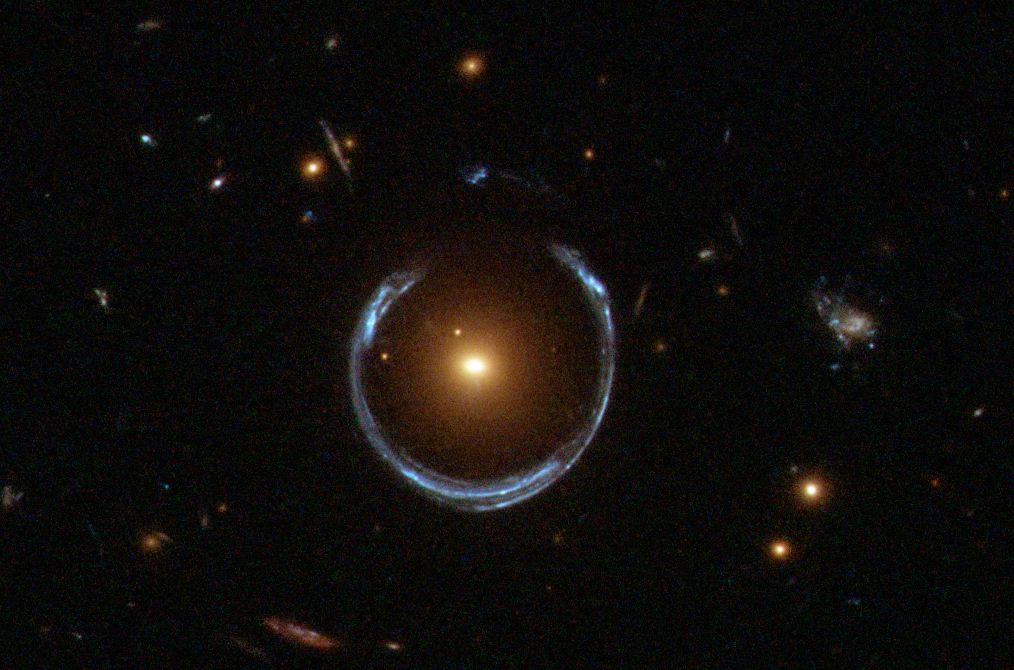
\includegraphics[trim={0cm, 2cm, 0cm, 0cm}, clip, height=4.5cm]{lensing_horseshoe}
 \end{subfigure}%
 \begin{subfigure}[t]{0.5\textwidth}
  \centering
  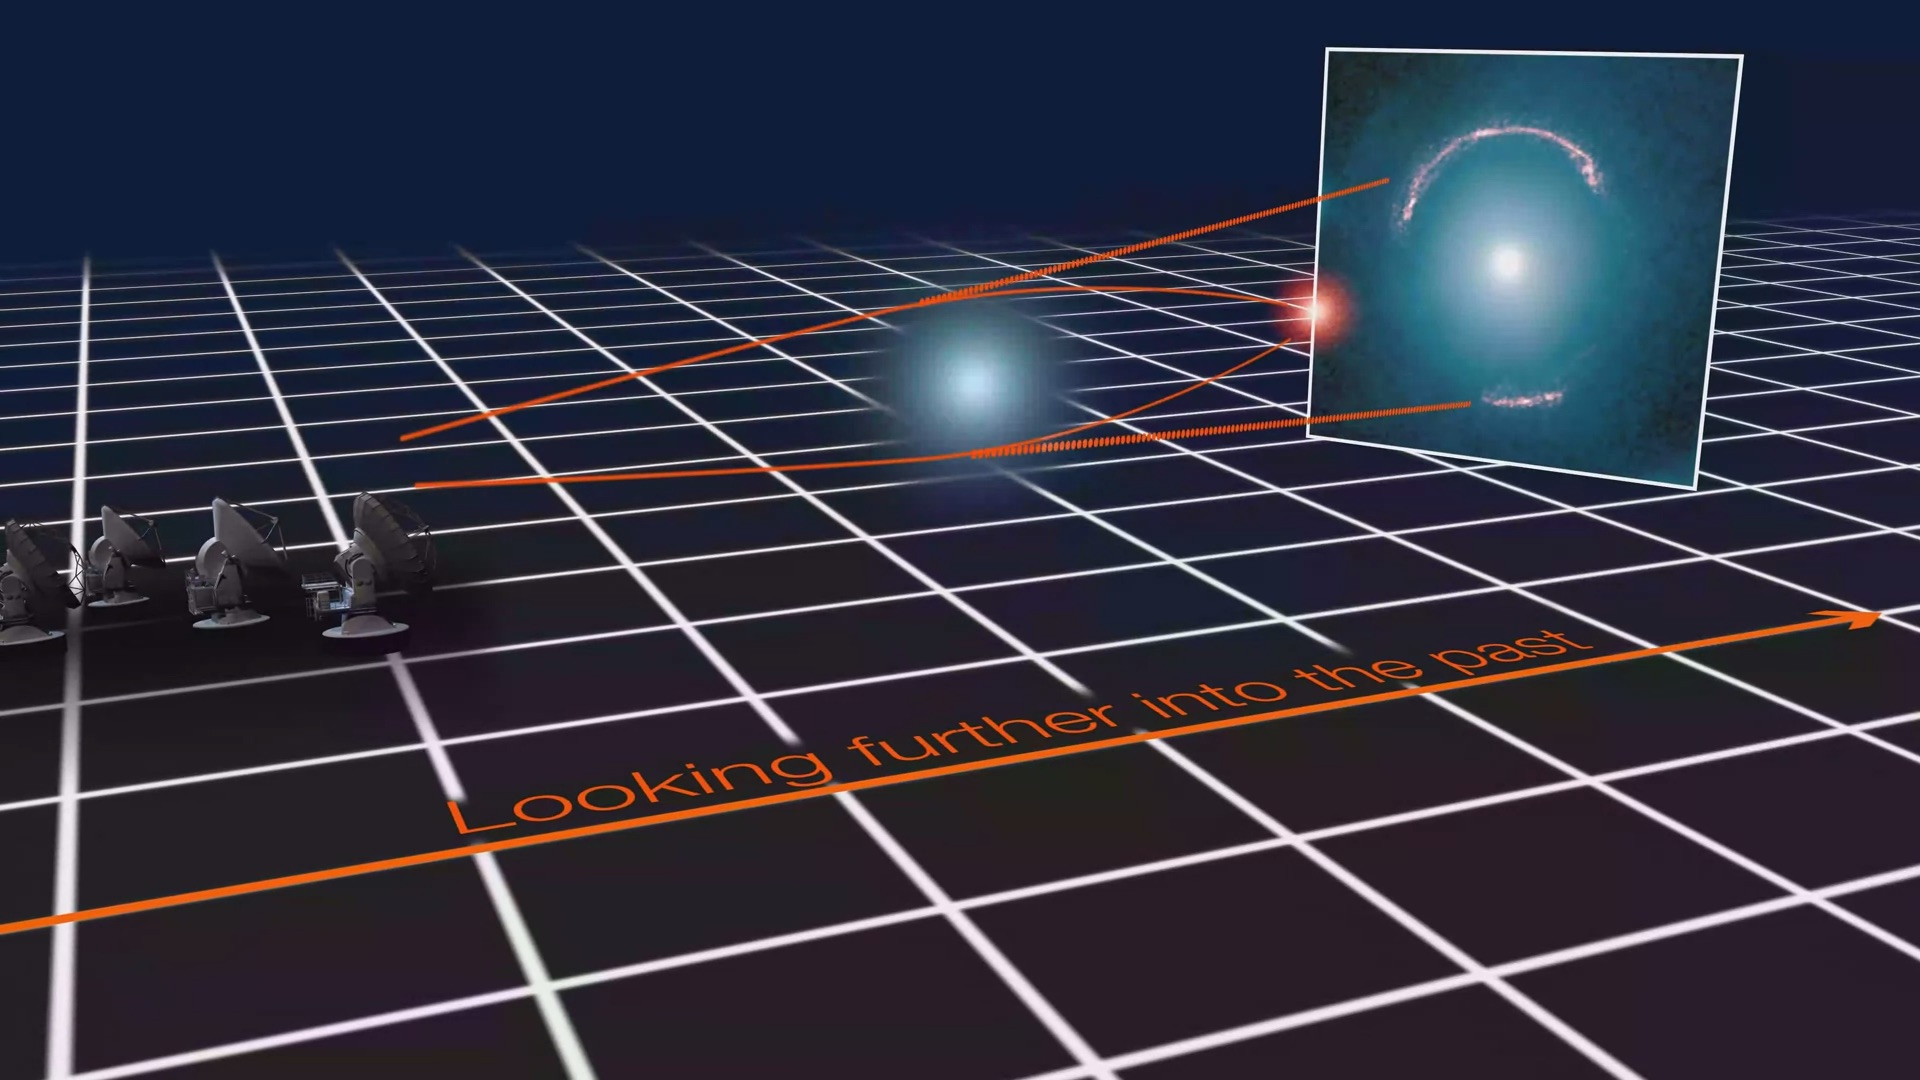
\includegraphics[trim={6cm, 0cm, 0cm, 0cm}, clip, height=4.5cm]{lensing_diagram}
 \end{subfigure}
 \caption[(left) A red galaxy distorts the light from a more distant blue galaxy to produce an Einstein ``horseshoe"
 ring.  (right)
 A diagram of strong lensing.]{(left) A red galaxy distorts the light from a more distant blue galaxy to produce an Einstein ``horseshoe"
 ring.  (right)
 A diagram of strong lensing.  The red source is bent by the blue lens, with the solid orange lines that connect
 to it representing the light's true trajectory.  The observer incorrectly views the source's
 position as indicated by the dashed orange lines, and the image behind them.  Image credit: (left) \citeref{ESAHubbleNASA2018}, (right)
 \citeref{ESO2018}.}
 \label{fig:lensing}
\end{figure}


In many astrophysical instances the light's deflection is much more subtle.  This is known as weak
lensing, and because the effects are fainter is more difficult to observe.  Whereas strong lensing results from radiation passing around
the lens, weak lensing is the passage of light through a gravitational field where tidal effects distort the shape of the image.  In the
latter the luminosity is often too low for a thorough analysis so
astronomers may only consider the source's shear.  However, because the size of the shear for weak lensing is small, systematic
effects from observation (e.g. atmosphere, instrument point spread function, noise, etc.) must be small and well
understood \citeref{Paolis2016}.  Furthermore,
because galaxies are generally elliptical, decoupling the true shape from the shear can be difficult to impossible.  Thus the
gravitational field is calculated statistically by randomly drawing galaxies from the known galaxy ellipticity distribution.  Since the
number of samples must equal the number of galaxies along the line of sight, this method is most effective when the number of galaxies is
large.

If the mass of the lens is well-known, the visible portion can be subtracted to yield its fraction of dark matter.  This can typically
be done for strong lenses as shown in \figref{fig:lensing} but is more difficult for weak.



\begin{figure}
    \centering
    \begin{subfigure}[t]{0.45\textwidth}
        \centering
        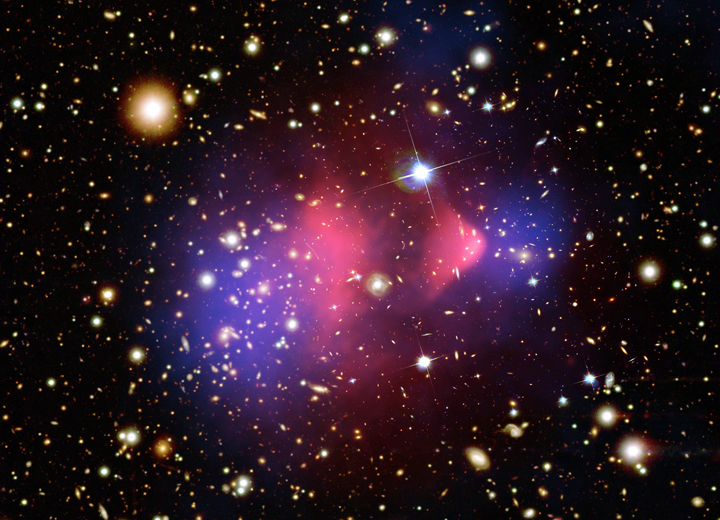
\includegraphics[height=4.5cm]{chandra_bullett_preview}
    \end{subfigure}%
    \begin{subfigure}[t]{0.45\textwidth}
        \centering
        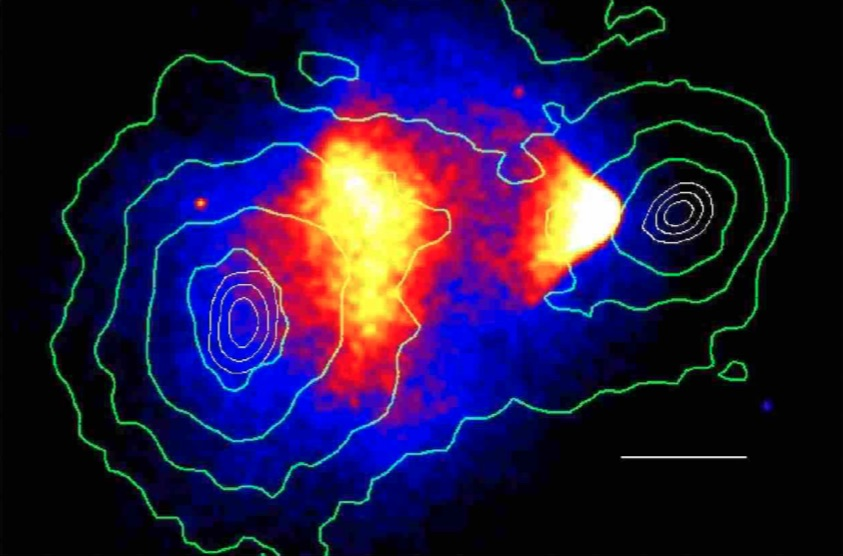
\includegraphics[height=4.5cm]{bullet_cluster_paper}
    \end{subfigure}
    \caption[X-ray emission from hot gas (pink) and mass centroids (blue) from gravitational lensing after
	collision of cluster 1E 0657-558.]{X-ray emission from hot gas (pink) and mass centroids (blue) from gravitational
	lensing after
	collision of cluster 1E 0657-558.  The white bar in the right panel represents 200 kpc at the cluster.  The separation
	between the colors provides evidence for Dark Matter.
	Image credit: (left) \citeref{Markevitch2006, Clowe2006}, NASA/CXC/CfA/STScIMagellan/U.Arizona/;
	Lensing Map: NASA/STScI; ESO WFI; Magellan/U.Arizona/D.Clowe et al. (right) \citeref{Clowe2006}.}
	\label{fig:bullet_cluster}
\end{figure}

A galaxy collision provides a unique setting to study dark matter.  1E0657-56, commonly known as the Bullet Cluster, is two galaxies that
passed through one another ${\sim}150$ million years ago at $4500_{-800}^{+1100}\ \mathrm{km\ s^{-1}}$
\citeref{Markevitch2004}.  \figref{fig:bullet_cluster} shows the x-ray map in pink and the mass
distribution from gravitational lensing measurements in blue in the left panel, and the mass contours in the right.  The separation of
mass from baryonic matter can be explained by dark matter.  As the galaxies collide intergalactic dust interacts
and heats up, creating x-rays and slowing their speed.  Because dark matter does not interact electromagnetically it moves
unimpeded by comparison, affected only by gravity.  In addition to providing evidence of dark matter, 1E0657-56 sets a limit on the
cross-section of dark matter self-interaction of ${<}\, 1\ \mathrm{cm^{2}\ g^{-1}}$ \citeref{Markevitch2004}.  It also provides evidence
against modified gravity (\secref{subsec:modified_gravity}) - an alternative theory to dark matter - since the observed mass distribution
lays outside of the luminous content.




%========
\subsection{Cosmic Microwave Background} \label{subsec:cmb}
The Cosmic Microwave Background (CMB) was accidentally discovered in 1965 by Arno Penzias and Robert Wilson, for which they received
the Nobel Prize \citeref{Penzias1965}.  It
is a remnant from shortly after (${\sim}380,000\ \mathrm{y}$, $z\sim1100$, $T\sim3000\ \mr{K}$) the Big Bang  and a near-perfect
blackbody at $2.725\ \mr{K}$ today (most precise measurement is $2.72548 \pm 0.00057\ \mr{K}$ \citeref{Fixsen2009}).  CMB photons
have been traveling freely since the time of last scattering $t_{\mathrm{ls}}$ - when electron-atom recombination in the early universe
was effectively complete, ending the period of (primarily) electron-photon scattering.

Deviations in the blackbody spectrum are small (root mean square of $\delta T/T \sim 10^{-5}$) and result from a number of
processes at $t_{\mathrm{ls}}$ that fluctuated throughout space.  A dipole anisotropy is due to
Earth's motion with respect to the comoving rest frame of the CMB \citeref{Smoot1991}.  Furthermore,
energy density perturbations would cause variations in gravitational potential $\delta \Phi$.  A
photon at a larger $\delta \Phi$ at $t_{\mathrm{ls}}$ would be blueshifted since as it moves its
potential decreases, while one at lower $\delta \Phi$ would be redshifted.  This is known as the
Sachs-Wolfe effect \citeref{Sachs1967}.  Details of additional effects, including intrinsic fluctuations and acoustic
oscillations, can be found in \citeref{Dodelson2003}.

\begin{figure}
\centering
\includegraphics[width=0.8\textwidth]{2015_SMICA_CMB_lower_memory}
\caption{CMB as observed by Planck.  Temperature deviations $\delta T/T \sim 10^{-5}$.  Image credit: \citeref{Planck2018}.}
\label{fig:planck_map}
\end{figure}


The CMB provides the most precise measurements on numerous cosmological parameters including $\Omega_{\mathrm{b}}$,
$\Omega_{\mathrm{dm}}$, $\Omega_{\Lambda}$, $\Omega_{\mathrm{r}}$, and $H_{0}$.  It has been charted by several satellites since
its
discovery, most recently by Planck \citeref{Plack2011}.  The CMB is shown in \figref{fig:planck_map},
where fluctuations are on the order of $10^{2} \mathrm{\mu K}$.  These fluctuations were caused by the
amount of each component - thus, by calculating the correlation function

\begin{equation}
%C(\theta) = \Big \langle \frac{\delta T}{T}( \hat{n}) \frac{\delta T}{T} ( \hat{n}^\prime) \Big \rangle
C(\theta) = \Big \langle \delta T( \hat{n}) \delta T(\hat{n}^\prime) \Big \rangle
\label{eq:cmb_corr_func}
\end{equation}

\noindent we can identify the cosmological makeup of the universe.  To do this we use

\begin{equation}
\delta T = \sum\limits_{l=0}^{\infty} \sum\limits_{m=-l}^{l} a_{lm}Y_{lm}(\theta, \phi)
\label{eq:cmb_delta_t}
\end{equation}

\noindent where $\delta T = T(\theta, \phi) - \langle T \rangle$ for a given $\theta , \phi$
on the map.  $Y_{lm}(\theta, \phi)$ are the spherical harmonics with coefficients $a_{lm}$
such that $\sum\limits_{l,m} |a_{lm}|^{2} = 1$.  Substituting \eqnref{eq:cmb_delta_t} into \eqnref{eq:cmb_corr_func} gives a correlation
function of

\begin{equation}
C(\theta) = \frac{1}{4 \pi} \sum\limits_{l=0}^{\infty} (2l + 1) C_{l} P_{l}(cos \theta)
\end{equation}

\noindent where $P_{l}$ are the Legendre polynomials and $C_{l} = \frac{1}{2l + 1} \sum\limits_{m=-l}^{l} a_{lm}$.  The
only unknown is $C_{l}$, which is typically given as the angular power spectrum
$D_{l}^{TT} \equiv l(l+1)C_{l}/2\pi$ as shown in \figref{fig:cmb_power_spectrum}.

\begin{figure}
%	\centering
	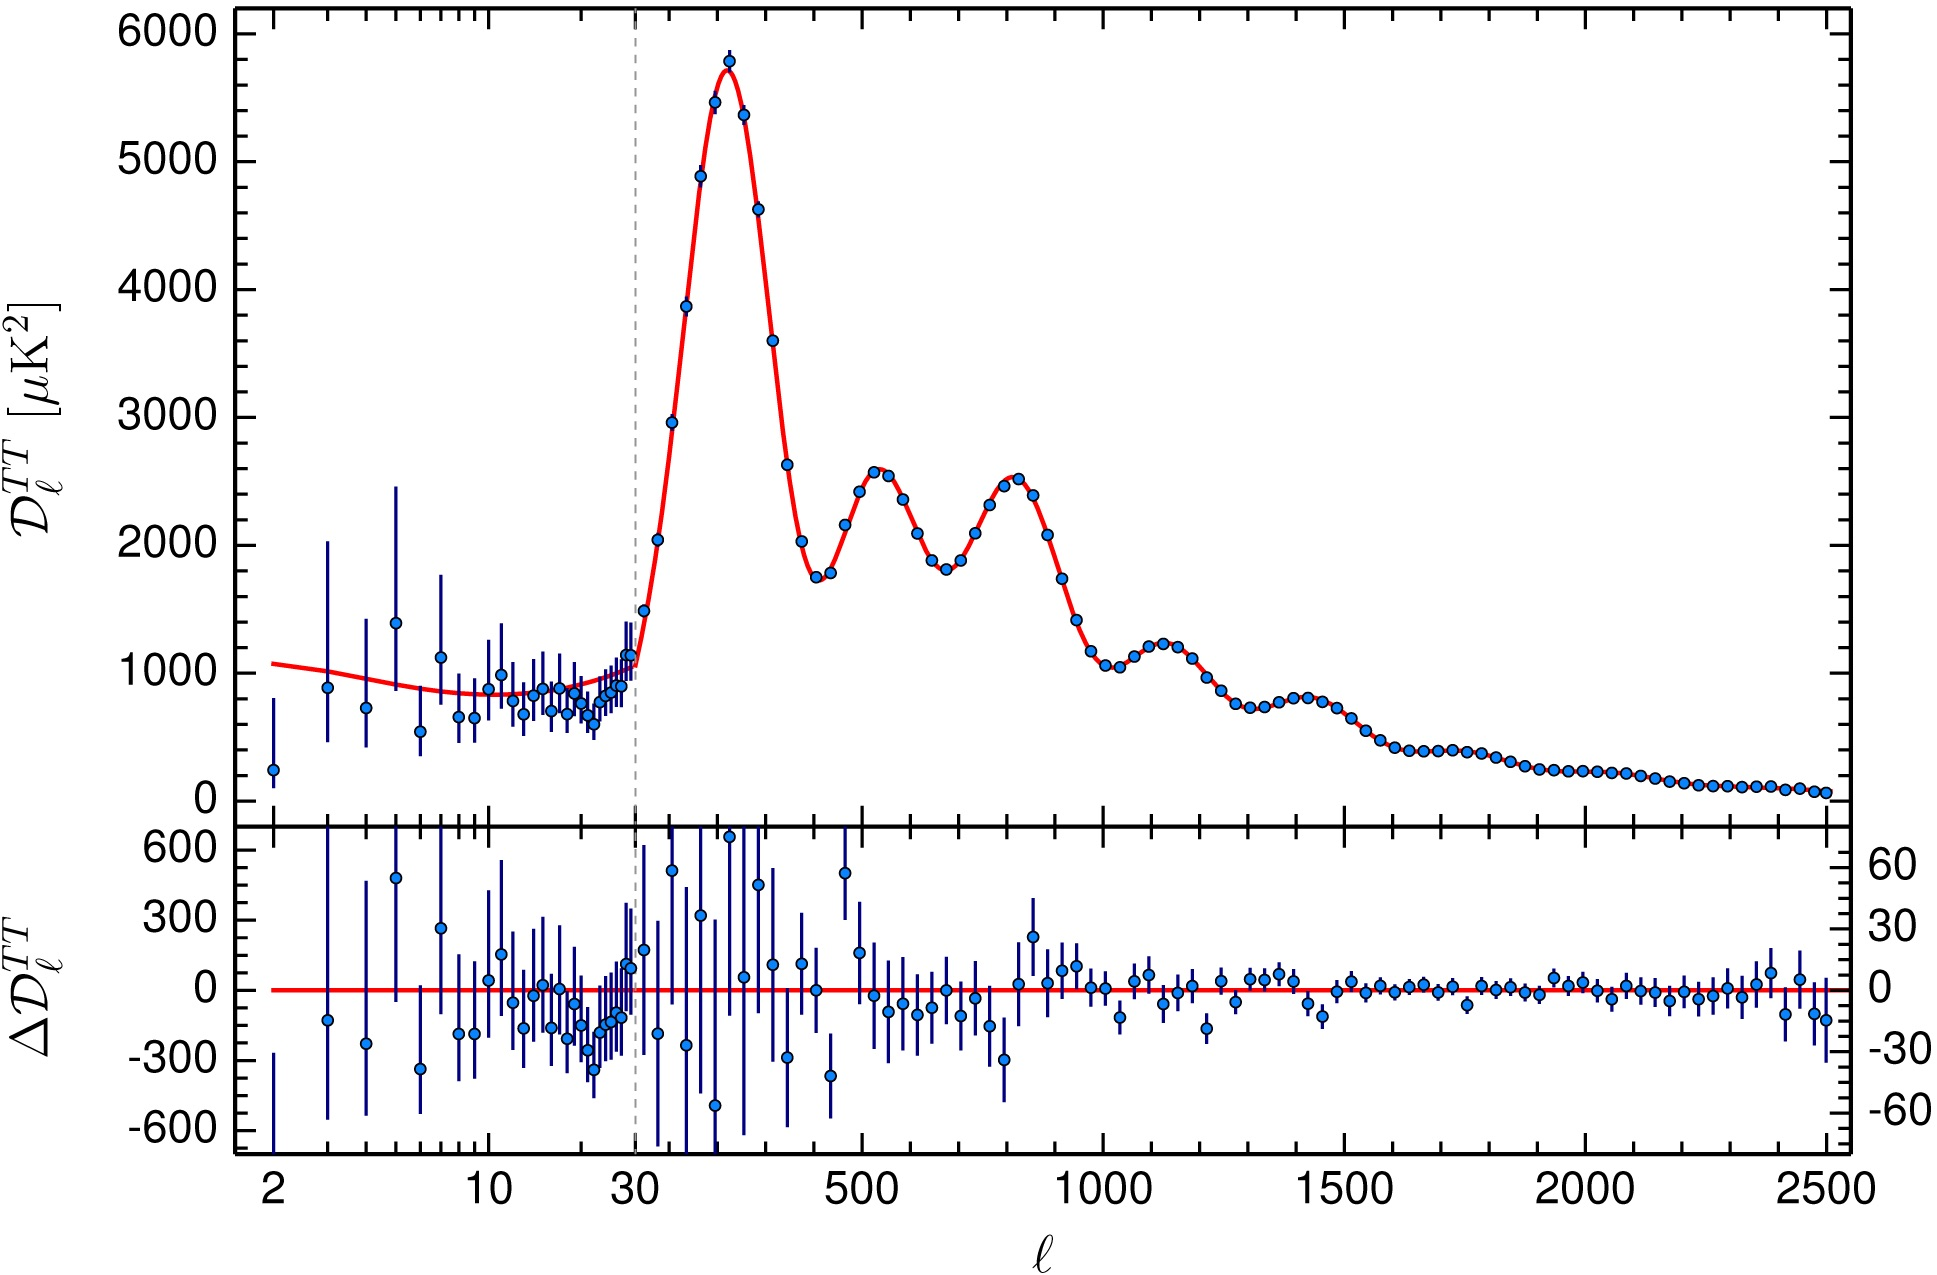
\includegraphics[width=0.8\textwidth]{cmb_power_spectrum}
	\centering
	\caption[Angular power spectrum for CMB from Planck using the $\Lambda$CDM model.]{Angular power spectrum for CMB from Planck using the
	$\Lambda$CDM model.  Residuals
	are shown in the bottom panel.  The model matches the data well at $l < 15$ and $l > 30$.  The horizontal axis changes from linear to
	logarithmic at $l = 29$ and is marked by the vertical dashed grey
	line. Image credit: \citeref{Planck2016}.}
	\label{fig:cmb_power_spectrum}
\end{figure}

Details about cosmological parameters including $\Omega_i$ are contained in the angular power spectrum (e.g. information on the curvature
is found in the first peak while the $\Omega_{\mathrm{b}}$ is derived from the ratio of the heights of the first two peaks).  The results
of the fit give $H_{0} = 67.81 \pm 0.92\ \mathrm{km\ s^{-1}\ Mpc^{-1}}$, $\Omega_{\Lambda} = 0.692 \pm 0.012$,
$\Omega_{\mathrm{b}} = 0.0484 \pm 0.0005$, $\Omega_{\mathrm{dm}} = 0.258 \pm 0.004$, and curvature density parameter
$\Omega_{k} \equiv 1 - \Omega_{\Lambda} - \Omega_{\mathrm{b}} - \Omega_{\mathrm{dm}} =  -0.005_{-0.017}^{+0.016}$.


%[5] Adams, F.C., Freese, K. & Guth, A.H. [1991], Phys. Rev. D43, 965.



%$\Omega_{m} = 0.308 \pm 0.012$
%$H_{0} = 67.81 \pm 0.92$
%$\Omega_{\Lambda} = 0.692 \pm 0.012$
%$\Omega_{b}h^{2} = 0.02226 \pm 0.00023$
%$\Omega_{c}h^{2} = 0.1186 \pm 0.0020$
%$N_{eff} = 3.046$
%$\Omega_{k} \equiv 1 - \Omega_{m} - \Omega_{\Lambda} = -0.005_{0.017}^{0.16}$ for $\Lambda CDM$

%========
%\subsection{Structure Formation} \label{subsec:structure}

%\endcsname

%====================================
\section[Dark Matter Candidates][Dark Matter Candidates]{Dark Matter Candidates}
\label{sec:dmcandidates}
Despite strong evidence for the existence of dark matter, there is little guidance for its composition.  Any dark matter candidate must
have a lifetime much larger than the age of the universe, be electrically
neutral, and have a small matter-dark matter cross section.  Of course, dark matter may constitute a class of particles so long as their
sum satisfies our observations of the universe.



%========
\subsection{Axions} \label{subsec:axions}
Charge conjugation and parity (CP) violation in strong interactions has never been observed, despite its allowance
by quantum chromodynamics (QCD).  This compels a theoretically unjustified fine tuning of the model, which
is known as the strong CP problem.  Originally hypothesized by Roberto Peccei and Helen Quinn in 1977, the
axion - a new standard model particle - offered a solution \citeref{Peccei1977}.  Shortly after it was
demonstrated that for an axion decay constant of $f_{\mathrm{a}} > 10^{12}$ axions would be overproduced in the
early universe and cause the axion density $\Omega_{\mathrm{a}} > 1 > \Omega_{\mathrm{dm}}$ \citeref{Preskill1983}.  However, if the
decay constant were ${\sim} 10^{12}$ the axion density parameter could be equivalent to $\Omega_{\mathrm{dm}}$.  Current mechanisms for
solving
the strong CP problem rely on invisible axion models Kim-Shifman-Vainshtein-Zakharov (KSVZ) \citeref{Kim1979, Shifman1980} and
Dine-Fischler-Srednicki-Zhitnitsky
(DFSZ) \citeref{Zhitnitsky1980, Dine1981}, marked along the yellow band in \figref{fig:axions}.  $f_{\mathrm{a}}$ is inversely
proportional to the axion mass $m_{\mathrm{a}}$.

\begin{figure}
\centering
\includegraphics[width=\textwidth]{axion_limits}
\caption{Axion-double photon coupling with respect to axion mass.  The shaded regions have been excluded by different
experiments.  Invisible axion models KSVZ and DFSZ are drawn along the yellow band.  Image credit: \citeref{Patrignani2016}.}
\label{fig:axions}
\end{figure}

%The axion
%mass $m_{a} = 57(10^{11}GeV/f_{a})\ \mu$eV, which gives a lower bound of $m_{a} \sim 5\ \mu$eV.

Because axions naturally offer an explanation for dark matter there are a number of DM experiments dedicated to
finding them.  Several operate under the Primakoff effect \citeref{Primakoff1951}, which states that electromagnetic fields should
transform
axions to photons and vice versa.  Cavity searches such as the Axion Dark Matter Experiment (ADMX) \citeref{ADMX2018} search the galactic
dark matter halo using a resonant microwave cavity inside a superconducting magnet
to convert axions at Earth into microwaves.  Others, like the CERN Axion Solar Telescope (CAST) search for axions produced in the Sun's
core from x-ray scattering off of protons and electrons \citeref{CAST2017}.  The experiment hopes to convert solar axions back into
x-rays.  The Cosmic Axion
Spin Precession Experiment (CASPEr) uses nuclear magnetic resonance (NMR) to detect nuclear spin precession frequencies that depend on
$m_{\mathrm{a}}$ \citeref{CASPEr2018}.  In addition axion-induced electronic recoils have been searched for in cryogenic detectors
including CDMS \citeref{CDMS2009}, EDELWEISS \citeref{EDELWEISS2013}, and XMASS \citeref{XMASS2013}.  The best electronic recoil coupling
limits to date were set by XENON100 in 2014 \citeref{Aprile2014}.


%========
\subsection{WIMPs} \label{subsec:wimps}
Weakly Interacting Massive Particles (WIMPs) are another favored candidate for dark matter.  As their name
suggests, they interact through the weak force so would be difficult to observe.  They
would behave similarly to neutrinos, which have a small cross-section and communicate only via the weak interaction.  They must also have
been produced early in the universe to account for observations of the CMB and galactic structures.

At the beginning of the universe the temperature was hot enough that particles could annihilate with their
antiparticle counterpart and produce new particles, maintaining equilibrium.  As the universe cooled each
particle underwent its own ``freeze-out'', after which they could no longer transform freely to other particles.  Using the
$\Lambda$CDM model the density of DM in the universe today is given by

\begin{equation}
\Omega_{\mathrm{dm}}h^{2} = \frac{3 \times 10^{-27}\ \mathrm{cm^{3}\ s^{-1}}}{\langle \sigma_{\mathrm{ann}} v \rangle}
\end{equation}

\noindent where $h \equiv H_0 / 100$ and $\langle \sigma_{\mathrm{ann}} v \rangle$ is
the thermally averaged self-annihilation cross section
for dark matter.  Assuming DM has a cross section and mass on the order of the weak scale,
it would give roughly the correct relic density of DM.  This is known as the ``WIMP miracle".

Another appealing argument for WIMPs is supersymmetry (SUSY), which is theorized to solve a number of problems
in the standard model.  Many SUSY models predict a heavy stable particle that would be weakly interacting (a favorite is the neutralino,
the supersymmetric partner of the neutrino).  This has historically been one of the favored arguments for WIMP dark matter.

%========
\subsection{Cold, Warm, or Hot} \label{subsec:hot_vs_cold}
An important property of dark is whether it was relativistic in the early universe, typically defined using the times of decoupling
from radiation and matter $t_{\mathrm{dec}}$ and matter-radiation equality (moment when density of matter and radiation are equivalent)
$t_{\mathrm{rm}}$.  Hot dark matter (HDM) would have been relativistic at $t_{\mathrm{dec}}$ and $t_{\mathrm{rm}}$.  Warm dark matter
(WDM) would have been relativistic at $t_{\mathrm{dec}}$
but not at $t_{\mathrm{rm}}$.  Cold dark matter (CDM) would have been non-relativistic at both.  Candidates for CDM include
WIMPs, axions, and primordial black holes while for WDM might be the gravitino.  Neutrinos are candidates for both
warm and hot dark matter, but measurements show their density is too small to account for $\Omega_{\mathrm{dm}}$.

Structure formation in the universe unravels the hot/warm/cold dark matter mystery.  Because the cosmological layout we observe
today came from fluctuations in the earliest moments after the Big Bang (\secref{subsec:cmb}) it contains the imprint of dark matter.

Relativistic energies of hot dark matter would smooth out density perturbations in what is known as free
streaming.  In this case the first structures to form would be superclusters, followed by smaller-scale
features.  Observations show that this is not the case; galaxies have been around since before the universe
was 1 billion years old ($z \sim 6$) and superclusters are just forming today \citeref{Ryden2003}.

CDM allows early density perturbations to persist, causing smaller structures to materialize first, which is
consistent with galaxy surveys between ${\sim} 1$ Mpc and the cosmological horizon.  At scales ${<}\, 1$ Mpc and
$M \sim 10^{11} \ M_{\odot}$ there are discrepancies, including under-dense cores for many galaxies that are DM-dominated
and significantly fewer satellite dwarf and small galaxies than predicted \citeref{Moore1999, Klypin1999}.  Possible
solutions to the latter may be that dwarf galaxies have merged, been stripped by tidal forces of larger galaxies, or
not accumulated enough baryonic matter to be visible \citeref{Simon2007}.

WDM has received a lot of interest since the problems with CDM were discovered.  Simulations have shown that
WDM would result in fewer subhalos, though explaining the other CDM model-observation disagreements has been less
successful \citeref{Bullock2017, Ogiya2017}.  However, because neutrinos have mass we know there
was at least some non-CDM in the early universe.

Despite problems with CDM it remains the most favorable model for dark matter.  One possible outcome is
there is a mix of CDM and WDM, but if that's the case CDM would make up the considerable bulk of dark matter.



\subsection{Modified Gravity}
\label{subsec:modified_gravity}
A different explanation for the disparity between the mass of ordinary matter and its behavior is an incomplete understanding of
gravity.  This
would suggest that Einstein's General Relativity works well at small distances but does not correctly explain large-scale
gravitation.  Since the incompatibility of current theory with observation would be resolved by proving the mysterious behavior is
a consequence of ordinary matter, dark matter would not be necessary.

Major evidence against modified gravity emerged in 2004 when the collision of two galaxies 1E0657-56 (Bullet Cluster) was observed
(\secref{subsec:gravitational_lensing}).  \citeref{Markevitch2004} reconstructed the mass distribution of the merger from gravitational
lensing measurements (\figref{fig:bullet_cluster}).  Their measurements required a significant fraction of the mass
distribution to be offset from the visible matter, consistent with collisionless dark matter halos passing through one another.  This
presented a problem for modified gravity, which was unable to justify this.

In 2018 the ultra-diffuse galaxy NGC1052-DF2 was observed to have $M_{\mathrm{halo}} / M_{\mathrm{stars}} \sim 1$, a factor of
roughly $400$
lower than expected \citeref{VanDokkum2018a, VanDokkum2018b}.  This poses a challenge to modified gravity - including modified Newtonian
dynamics
(MOND), a popular theory that has successfully predicted a number of galactic phenomena \citeref{Milgrom1983} - since a large
gravitational
field does not appear to exist around the baryonic matter.  However, several theories have claimed this may be compatible with their
expectations due to its proximity to its massive host galaxy NGC1052 and large uncertainties on some of the measurements by
\citeref{VanDokkum2018a, Famaey2018, Moffat2018}.  Under the dark matter hypothesis, a galaxy without DM has implications outside
this field - e.g. current models of structure formation cannot explain this \citeref{Abraham2018, Ogiya2018}.  Two recent
papers found conflicting results when studying the 175 SPARC
galaxies \citeref{Lelli2016}.  The first was in agreement with MOND using gaussian priors centered around values given by SPARC by
setting
their uncertainty to observational errors \citeref{Li2018}.  The second included an additional 18 galaxies from THINGS
\citeref{deBlok2008} and with flat priors excluded MOND
at $10 \sigma$ \citeref{Rodrigues2018}.  Ultimately, additional measurements and improved statistics are needed to better
quantify NGC1052-DF2, but confirmation of missing dark matter would strongly constrain theories of modified gravity.


%====================================
\section[WIMP Detection Methods][WIMP Detection Methods]{WIMP Detection Methods}
\label{sec:detection}

There are three methods for detecting WIMPs.  The first is using particle colliders where standard model (SM) particles would interact and
create DM (\secref{subsec:colliders}).  The second is via indirect detection, where DM would annihilate into SM particles, with the hope
that they would be detectable
on Earth (\secref{subsec:indirect}).  Experiments look in high-density regions of the universe where higher concentrations of dark matter
should be present.  The third method is by direct detection in which DM would scatter off SM matter and produce
a signal that could be observed (\secref{subsec:direct}).  These methods are outlined in \figref{fig:detection_methods}.

\begin{figure}
\centering
\includegraphics[width=0.6\textwidth]{detection_methods}
\caption[Dark matter detection methods.  Image credit: \citeref{Bi2013}.]{Dark matter detection methods.  High energy
particle collisions may create dark matter that would result in missing transverse
energy (bottom).  Indirect detection looks for signatures (e.g. neutrinos, photons) of possible dark matter annihilation in the
universe (top).  Direct detection experiments search for signs of dark matter scattering off Standard Model particles (right).  Image
credit: \citeref{Bi2013}.}
\label{fig:detection_methods}
\end{figure}

 %========
\subsection{Colliders} \label{subsec:colliders}
One mechanism that might lead to the discovery of WIMP dark matter is particle-antiparticle
annihilation.  This could be observed at particle colliders where energies can exceed
several TeV, producing dark matter particle-antiparticle pairs.  Though they would escape undetected, they could be measured through
missing transverse energy (MET) using momentum conservation.  The
Large Hadron Collider (LHC) is investigating the quark sector with energies
exceeding 10 TeV, while the Large Electron-Positron (LEP) Collider is doing so for leptons at
${\sim} 200$ GeV.  Both experiments are more competitive at lower energies than noble gas experiments (\secref{subsec:noble_gas}),
particularly for spin-dependent searches \citeref{Fox2011, Alpigiani2017}.  MET observations alone would not prove the existence of dark
matter but would need
indirect or direct experiments to validate their results.  However, it would still be extremely useful in narrowing the search region.

\begin{figure}
\centering
\includegraphics[width=0.8\textwidth]{collider_diagram}
\caption{Diagram of a collision at the LHC.  Image credit: \citeref{CERN2018}.}
\label{fig:collider}
\end{figure}


 %========
\subsection{Indirect Detection} \label{subsec:indirect}
Indirect detection looks for signatures of dark matter by observing standard model particles.  Observables
may come from dark matter annihilation, wherein two DM particles annihilate and produce standard model
gamma-rays or other particle-antiparticle pairs.  Alternatively, if DM is unstable (albeit with a very long half-life) it may decay into
standard model particles that can be detected.

Indirect experiments look at regions where they expect a large number of interactions.  The local
dark matter density is estimated to be 0.2-0.56 GeV cm$^{-3}$ \citeref{Read2014} and experiments are observing
the Sun hoping to measure a WIMP-induced high energy neutrino flux \citeref{Ellis1988}.  Other theories suspect
DM annihilation in high-density regions of the universe such as the galactic halo would produce
antiprotons, positrons, and gamma-rays that would be detectable from Earth.  Because the galaxy's center
has a large flux of cosmic rays it is difficult to distinguish possible dark matter from other astrophysical
sources.  Nearby (${\sim} 50$ kpc) dwarf spherical
galaxies have become an attractive target where star formation regions have low $\gamma$-ray backgrounds \citeref{Zitzer2016}.

$\gamma$-rays need to be measured in space because in the relevant energy range (GeV to TeV) photons interact
with matter via $e^{+}e^{-}$ pair production (\figref{fig:phot_atten}), and are unable to pass through Earth's atmosphere.  However,
ground-based detectors can look for signatures such as showers of secondary particles and their Cerenkov
light as they pass through the atmosphere \citeref{Bertone2005}.

% for Ellis1988 reference listed above get their references 6 and 7 and maybe 8 for citations, need access to PRL


 %========
\subsection{Direct Detection} \label{subsec:direct}
Direct detection mainly looks for low energy (${\sim} 1 \mdash 100$ keV) nuclear recoils (somes theories predict DM-lepton
interactions,
but they are not discussed here) \citeref{Kopp2009}.  The dark matter halo of a galaxy is normally assumed to be an isothermal
single-component sphere with an isotropic Maxwell-Boltzmann velocity distribution function
($f(\vectlett{v}) \propto \mathrm{exp}(-|\vectlett{v}|^2 / v_0^2)$) \citeref{Bhattacharjee2013}, though there is not a consensus on
whether this is the correct velocity parameterization
\citeref{Diemand2004, Kuhlen2009}.  This is known as the Standard Halo Model (SHM).  Given that the majority of dark matter must be
non-relativistic (\secref{subsec:hot_vs_cold}), the differential recoil spectrum is calculated as \citeref{Undagoitia2016}

\begin{equation} \label{eq:dr_de}
\frac{dR}{dE}(E, t) = \frac{\rho_{\chi}}{m_{\chi}m_{\mathrm{A}}} \int_{v_{\mathrm{min}}}^{v_{\mathrm{esc}}}
v f(\vectlett{v}, t) \frac{d\sigma}{dE}(E, t)\ d^{3}\vectlett{v}
\end{equation}

\noindent where $\rho_{\chi} = 0.2 \mdash 0.56\ \mathrm{GeV\ cm^{-3}}$ is the local dark matter density (\secref{subsec:indirect}),
$m_{\chi}$ is the mass of a
dark matter particle, $m_{\mathrm{A}}$ is the mass of the target element, $v_{\mathrm{esc}}= 533_{-41}^{+54}\ \mathrm{km\ s^{-1}}$
\citeref{Piffl2014} is the escape velocity for WIMPs from the
galaxy, $f(\vectlett{v}, t)$ is the local velocity dispersion, and $\frac{d\sigma}{dE}(E, t)$ is the nucleon-DM differential
cross-section.  $v$ is the velocity of the dark matter in the rest frame of the detector.  The minimum velocity that will produce
a recoil of energy E is

\begin{equation}
v_{\mathrm{min}} = \sqrt{\frac{m_{\mathrm{A}} E}{2 \mu^{2}}}
\end{equation}

\noindent where $\mu_{\mathrm{A}} = m_{\mathrm{A}} m_{\chi} /( m_{\mathrm{A}} + m_{\chi})$ is the reduced WIMP-nucleus mass.

For WIMP searches most experiments look for spin-independent (SI) or spin-dependent (SD) interactions.  For spin-independent all nucleons
contribute equally.  For spin-dependent, atoms must have an odd number
of protons or neutrons since only unpaired nucleons contribute to the search.  The differential cross-section can then be written as

\begin{equation} \label{eq:diff_sigma_si}
\frac{d \sigma}{dE} = \frac{m_{\mathrm{A}}}{2 \mu_{\mathrm{A}}^{2} v^{2}} \big( \sigma_{\mathrm{SI}}^{(0)} F_{\mathrm{SI}}^{2}(E) +
\sigma_{\mathrm{SD}}^{(0)} F_{\mathrm{SD}}^{2}(E) \big)
\end{equation}

\noindent where $\sigma_{\mathrm{SI}}^{(0)}$ and $\sigma_{\mathrm{SD}}^{(0)}$ are the cross sections at zero momentum for
spin-independent and spin-dependent DM.  $F_{\mathrm{SI}}^{2}(E)$ and $F_{\mathrm{SD}}^{2}(E)$ are the form factors, which
account for the cross section's decrease with increasing energy \citeref{Lewin1996}.  Spin-dependence is no longer discussed but details
are found in \citeref{Lewin1996}.  The SI form factor is
the Fourier transform of the mass density ground state, and for the parameterization given in \citeref{Helm1956} is

\begin{equation}
F_{\mathrm{SI}} = \frac{3 j_{1}(qr_{\mathrm{n}})}{qr_{\mathrm{n}}} e^{-(qs)^{2}/2}
\end{equation}

\noindent where $j_1(q r_{\mathrm{n}})$ is a Bessel function of the first kind, $q = \sqrt{2m_{\mathrm{A}}E}$ is the momentum,
$r_{\mathrm{n}} = \sqrt{1.2A^{2/3} - 5s^{2}}$, and $s \sim 1$ fm is a measure of the nuclear skin \citeref{Lewin1996, Engel1991}.  The
cross section is given by

\begin{equation} \label{eq:sigma_si}
\sigma_{\mathrm{SI}}^{(0)} = \sigma_{\mathrm{p}} \frac{\mu_{\mathrm{A}}^{2}}{\mu_{\mathrm{p}}^{2}} \frac{\big[ Z f_{\mathrm{p}} +
(A - Z) f_{\mathrm{n}} \big]^{2}}{(f_{\mathrm{p}})^{2}}
\end{equation}

\noindent where $\sigma_{\mathrm{p}}$ is the cross section of a proton, $Z$ is the number of protons, and $\mu_{\mathrm{p}}$ is
the WIMP-nucleon reduced mass. $f_{\mathrm{p/n}}$ is the coupling strength for protons and neutrons, which are assumed to be
equivalent (see \citeref{Yaguna2017} for $f_{\mathrm{p}} \neq f_{\mathrm{n}}$).  Substituting \eqnref{eq:sigma_si} into
\eqnref{eq:diff_sigma_si} gives a spin-independent differential cross-section of

\begin{equation}
\frac{d \sigma}{dE} = \frac{m_{\mathrm{A}} \sigma_{\mathrm{p}}}{2 \mu_{\mathrm{p}}^{2} v^{2}}
 A^{2} \big| F(E) \big |^{2}
\end{equation}

\noindent This gives the differential rate as 

\begin{equation}
\frac{dR}{dE} = \frac{\rho_{\chi} A^{2} \sigma_{\mathrm{p}}}{2 m_{\mathrm{\chi}} \mu_{\mathrm{p}}^{2}}
  \big| F(E) \big |^{2} \int_{v_{\mathrm{min}}}^{v_{\mathrm{esc}}}
\frac{f(v)}{v}\ dv
\label{eq:dr_de_final}
\end{equation}

\noindent A direct detection experiment that is sensitive between energies $E_{\mathrm{min}}$ and $E_{\mathrm{max}}$ will measure
the number of signals over a time $T$ for their target mass $M$ as

\begin{equation} \label{eq:counts}
N ( m_{\chi}, \sigma) = T \times M \times \int_{E_{\mathrm{min}}}^{E_{\mathrm{max}}} \frac{dR}{dE} dE
\end{equation}

\noindent \eqnref{eq:dr_de_final} and \eqnref{eq:counts} state that the sensitivity of an experiment improves linearly with time and
target mass, but quadratically with $A$.  This makes the atoms or molecules of the target mass an important consideration when
designing a direct detection experiment.

%For SD interactions the cross-section is

%\begin{equation}
%\sigma_{0}^{\mathrm{SD}} = \frac{32}{\pi} \mu_{\mathrm{A}}^{2} G_{\mathrm{F}}^{2} \big[ a_{\mathrm{p}} \langle S^{\mathrm{p}} \rangle +
%a_{\mathrm{n}} \langle S^{\mathrm{n}} \rangle \big] \frac{J + 1}{J}
%\end{equation}

%\noindent where $G_{\mathrm{F}}$ is the Ferm coupling constant, $a_{\mathrm{p/n}}$ is the coupling constants, and $J$ is
%the total nuclear spin.




% https://journals.aps.org/rmp/abstract/10.1103/RevModPhys.28.214 for distribution of WIMP scatters assumed to be same
% as charge distribution derived from electron and muon scattering 


%correctly describes DM velocity
%as discussed in \secref{subsec:dynamics} assume the WIMP velocity the Maxwell-Boltzmann distribution



%Because current theory
%predicts the DM distribution to be in a halo around the galaxy (\secref{subsec:dynamics}), DM particles should
%be passing through Earth and - if they're WIMPS - interact with the nuclei of standard model atoms.



%The
%energy deposited in such a collision would be manifested as scintillation, excitation (nucleus or electron),
%ionization, or phonons.




%====================================
\section[Direct Detection Experiments][Direct Detection Experiments]{Direct Detection Experiments}
\label{sec:direct_detect}
When a moving particle scatters off an atom or molecule that is by comparison somewhat stationary it transfers some of its
energy.  The energy gained by the atom will cause three effects.  The first is the atom's translational energy might rise (heat) and
produce phonons that propagate across the medium.  The second is electrons may be excited to higher energy orbitals, and generate
photons
as they quickly de-excite.  The third is the atom may be ionized, after which the freed electrons may recombine with their parent ion
and emit photons or escape.  Direct detection experiments can probe each of these effects, and many are able to measure two of the three
simultaneously.  The different energy channels can be seen in \figref{fig:energy_channels}.

\begin{figure}
\centering
\includegraphics[width=0.8\textwidth]{energy_channels}
\caption{Energy channels.  Image credit: \citeref{Undagoitia2016}.}
\label{fig:energy_channels}
\end{figure}
 
Direct detection experiments look for events outside of their expected background.  This requires a comprehensive
understanding of the detector background to ensure any ``anomalous'' events do not come from mis-modeling and a false discovery is
claimed.  Different approaches may be
used for different methods of detection.  For some experiments major efforts are going into screening the radioactivity of
potential materials.  Radioactivity from outside of the detector may be shielded (using e.g. water, lead).  Finally, there may be
backgrounds that are intrinsic to the target material.

 
Even with a priori screening, effective shielding, and reducing intrinsic contaminants background events are inevitable.  Identifying a
signal will be difficult if the signal-to-background ratio is small.  This is because
an experiment with a large background will report an excess with less significance than one with a low background, i.e. a detector with a
10 event
background can make a stronger claim on an excess of 5 events than one with 100.  In 1986 it was proposed
that due to the Earth's motion around the Sun there should be a modulation in signal \citeref{Drukier1986}.  Thus
detectors could look for an annual variation in event rate that peaks in May, when the Earth's velocity around the
Sun aligns with to the Sun's velocity around the galaxy.

\begin{figure}
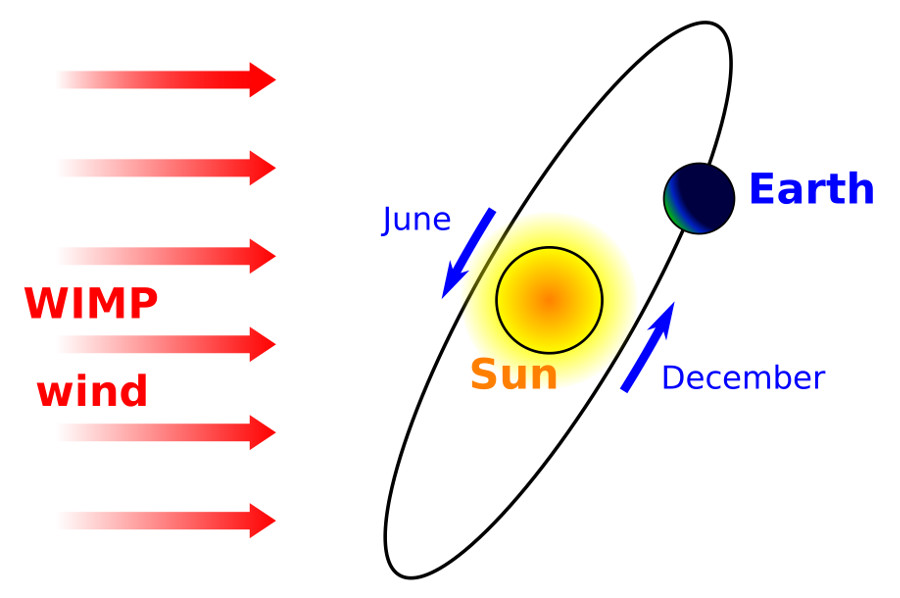
\includegraphics[width=0.6\textwidth]{wimp_wind}
\caption[Orientation of the Earth's rotation around the Sun.  The change in alignment of the Earth's and Sun's velocities causes the
amount of dark matter passing through the Earth to change, appearing as a ``WIMP wind'' with a 1-year period.  Image credit:
\citeref{Freese2013}.]{Orientation of the Earth's rotation around the Sun.  The change in alignment of the Earth's and Sun's velocities causes the
amount of dark matter passing through the Earth to change, appearing as a ``WIMP wind'' with a 1-year period.  The annual modulation
should be present for any DM velocity distribution as long as it does not align with that of the Sun.  Image credit:
\citeref{Freese2013}.}
\label{fig:direct_detect_modulation}
\end{figure}
 
  
 
 %========
\subsection{Superheated Liquid Detectors}
\label{subsec:bubbles}
Superheated liquid detectors are the most sensitive to WIMP masses in the tens of $\mathrm{GeV/c^2}$ range.  Their limits for
spin-independent
WIMPs are not as stringent as dual-phase noble gas detectors (\secref{subsec:noble_gas}), but for a number of years they have
consistently provided the strongest constraints in the spin-dependent WIMP-proton sector \citeref{PICO2017}.  Their strong
sensitivity comes from using fluorinated
halocarbons, since $^{19}$F is the only stable isotope and its unpaired proton
almost always carries 1/2 spin \citeref{Ellis1991, PICASSO2012}.

At ambient temperatures and pressures fluorinated halocarbons are in a metastable state.  A colliding particle will transfer some of its
heat, which can result in nucleation that is observed acoustically or optically.  By varying the temperature and pressure settings
superheated detectors can reduce $\gamma$ and $\beta$ interactions by a factor of 10$^{9}$, making them a great candidate for a
spin-dependent dark matter discovery.

Superheated detector collaborations include Project In CAnada to Search for Supersymmetric Objects (PICASSO) \citeref{PICASSO2017},
Chicagoland Observatory for Underground Particle Physics (COUPP) \citeref{COUPP2012},
PICO (merged from PICASSO and COUPP) \citeref{PICO2017}, Superheated Instrument for Massive ParticLe Experiments (SIMPLE)
\citeref{SIMPLE2012}, and Materia OSCura A Bolle (MOSCAB) \citeref{MOSCAB2017}.  \figref{fig:sd_limits} shows the exclusion plot of
spin-dependent WIMP-proton cross sections.


\begin{figure}
 \centering
 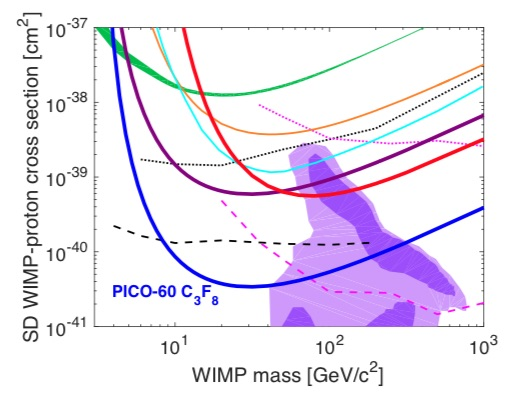
\includegraphics[width=0.8\textwidth]{spin_dependent_limits}
 \caption[Spin-dependent WIMP-proton cross-section 90\% C.L. limits.]{Spin-dependent WIMP-proton cross-section 90\% C.L. limits for PICO-60
 C$_{3}$F${_8}$ (thick blue, \citeref{PICO2017}), PICO-60 CF$_{3}$I (thick red,
 \citeref{PICO2016a}), PICO-2L (thick purple, \citeref{PICO2016b}), PICASSO (green, \citeref{PICASSO2017}), SIMPLE (orange,
 \citeref{SIMPLE2014}), and PandaX-II (cyan, \citeref{PandaXII2016a}).  Indirect limits from IceCube
 (dashed and dotted pink, \citeref{IceCube2017}) and SuperK (dashed and
 dotted black, \citeref{SuperK2011, SuperK2015}) for $b$ quark (dotted) and $\tau$ lepton (dashed)
 annihilation are shown.  The shaded purple region is constrained parameter space for the minimal
 supersymmetric model from \citeref{Roszkowski2007}.
 Image credit: \citeref{PICO2017}.}
 \label{fig:sd_limits}
\end{figure}

%When superheated liquid detectors were first considered for WIMP detectors there were some crucial points
%that needed to be addressed.  The downtime of such a detector was high because the temperature
%For WIMP searches modifications had to be made from the original
%devices including increased stability for near-continuous operation and operation as a counting experiment
%\citeref{Pullia2014}.

 %========
\subsection{Scintillation Crystals}
\label{subsec:crystals}
Another target for DM searches is highly radiopure scintillating crystals.  Typically sodium iodide (NaI) or cesium iodide (CsI) is
chosen, with NaI being the most common.  Their sensitivity to SI
and SD DM, low energy threshold, room temperature operability, and ability to run over long periods of time
make them an attractive option.  Doping these crystals with thallium increases the yield and shifts the wavelengths of the emitted light,
making the crystals
more transparent and improving phototube detection efficiency \citeref{Undagoitia2016}.  However, trace amounts of radioactive elements
are present in NaI(Tl) crystals \citeref{DAMALIBRA2008}.  The 3 keV x-ray/Auger electron from the decay of
$^{40}$K to \ce{^{40}Ar} through electron capture is particularly concerning because it lays in the region of interest.  In addition a
flat background is produced by \ce{^{87}Rb} and the $^{238}$U and $^{232}$Th decay chains.  Additionally, the features of the
scintillation
do not change for different types of interactions (e.g. $\gamma$-ray, neutron), so particle discrimination is not possible, with the
excepting of rejecting events with multiple scatters.  Thus differentiating between background and signal on an event by event basis is
not possible.  This has made improved radiopurity an increasingly important goal \citeref{Shields2015}.

\begin{figure}
\centering
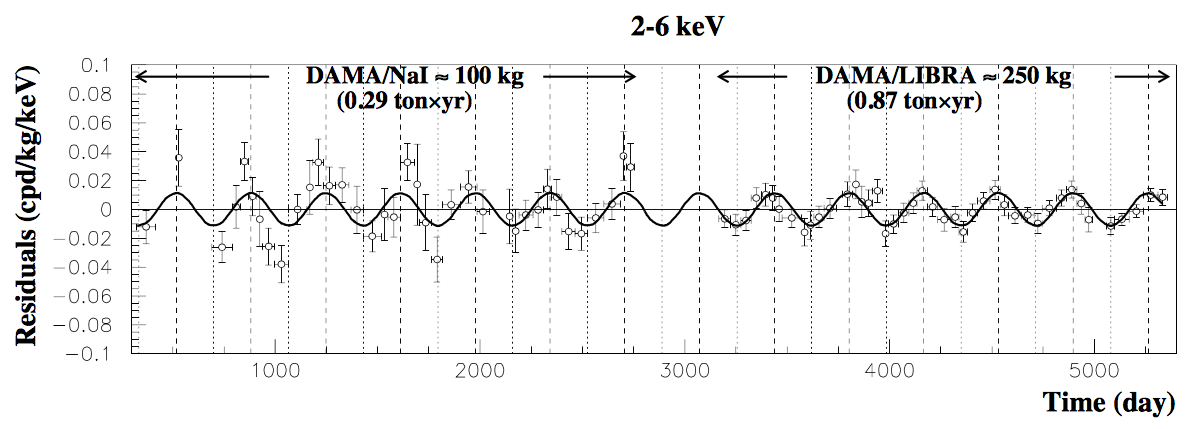
\includegraphics[width=\textwidth]{DAMAModulation}
\caption[Residual event rate between 2-6 \kevee as measured by DAMA/NaI and DAMA/LIBRA.  A fit of
$A \cos \lbrack \omega (t - t_{0}) \rbrack $ where $t_{0} = \mathrm{June\ 2nd}$ and $A$ is the best-fit amplitude is overlaid, with vertical
dashed lines corresponding to expected
maxima.]{Residual event rate between 2-6 \kevee as measured by DAMA/NaI and DAMA/LIBRA.  A fit of $A \cos \lbrack \omega (t - t_{0}) \rbrack$
where
$t_{0} = \mathrm{June\ 2nd}$ and $A$ is the best-fit amplitude is overlaid, with vertical dashed lines corresponding to expected
maxima.  For 14 years they have observed an annual
modulation with $9.3\sigma$.  Claiming this modulation is due to dark matter is controversial, as they are unable to
discriminate between different interaction types and a number of experiments have surpassed their sensitivity with no significant
findings.  Image credit: \citeref{Bernabei2013}.}
\label{fig:dama}
\end{figure}

The DAMA/NaI and its successor DAMA/LIBRA experiments are located underground at the Laboratori Nazionali del Gran Sasso (LNGS) in
L'Aquila, Italy.  They use NaI(Tl) crystals, which allows them to be sensitive to both low- (Na) and high-mass (I) WIMPs
\citeref{DAMALIBRA2008}.  For over 14 annual cycles they have observed an annual modulation in the
2-6 \kevee (\secref{subsubsec:tpcs_signals_energy})
range with 9.3$\sigma$ \citeref{DAMA2013}.  This corresponds to WIMP masses of $10 \mdash 15\ \mathrm{GeV/c^2}$ for sodium-scatters
and $60 \mdash 100\ \mathrm{GeV/c^2}$ for iodine.  Their results are shown in \figref{fig:dama}.  Spin-independent, spin-dependent or
mixed coupling \citeref{Bernabei2001} and inelastic scattering \citeref{Bernabei2002} WIMPs 
have been considered.  Because NaI(Tl) cannot distinguish scatterings of different
particles there is doubt on whether their signal
is caused by WIMPs, or even dark matter.  Furthermore, since they cannot specify if the interactions are with nuclei or electrons,
alternative dark matter
electron-coupling models \citeref{Bernabei2006} have been examined.  Their results are controversial because other experiments
have surpassed the DAMA/LIBRA sensitivity and see no signal \citeref{Aprile2017a}.  This has prompted theories to explain the annual
modulation via
Standard Model particles.  Hypotheses include known variation in muon flux due to changing stratosphere temperatures, which exhibits
annual modulation with a phase similar to DAMA/LIBRA's findings \citeref{Blum2011}, an incomplete understanding of neutron backgrounds
\citeref{Ralston2010}, or using a combination of muon-induced neutrons and solar neutrinos \citeref{2014Davis} (this
has been received pushback in \citeref{Barbea2014, Klinger2015}).  The Sodium iodide with Active Background REjection (SABRE) experiment
is being constructed at LNGS and plans on beginning to take data by the end of 2018 \citeref{Shields2015, SABRE2018}.  By using the same
technology and location they will be the first experiment to directly challenge DAMA/LIBRA.

 %========
\subsection{Germanium Detectors}
\label{subsec:germanium}
High purity germanium (HPGe) detectors measure ionization and offer exceptional energy resolution.  Like scintillation crystals,
(\secref{subsec:crystals}) they can reach very low energies (${\sim} 0.5\ \mathrm{keV}$), making them a promising candidate for low-mass
WIMP (${\sim} 10\ \mathrm{GeV/c^2}$) detection.  HPGe cannot differentiate nuclear recoils from electronic, but
p-type doped detectors have a dead layer on the surface and can use the
pulse rise time to reject background surface events.  In 2010 the Coherent Germanium Neutrino Technology (CoGeNT) experiment
announced it observed an annual modulation similar to DAMA/LIBRA \citeref{CoGeNT2010}.  After continued observation they found the
modulation had a best-fit
WIMP mass of $m_{\chi}\sim 8\ \mathrm{GeV/c^2}$ at $2.2\sigma$ \citeref{CoGeNT2014}.  However, subsequent analyses with
different
background assumptions showed this significance fell well below 1.7$\sigma$ \citeref{Aalseth2014, Davis2014}.  The China Dark matter
EXperiment (CDEX) uses the same setup as CoGeNT and found contradictory results \citeref{CDEX2014}, as did CDMS II for nuclear recoils
only \citeref{CDMS2012}.


%========
\subsection{Cryogenic Bolometers}
\label{subsec:bolometers}
Cryogenic bolometers are typically cooled to $10 \mdash 100$ mK so they can detect phonons, allowing a low energy threshold and
outstanding energy resolution.  The Cryogenic Dark Matter Search (CDMS) collaboration uses silicon and germanium detectors to
measure phonons
and ionization.  The ionization-to-phonon ratio is used for discrimination where less than 1 in $10^{6}$ of all electronic recoil events
fail to be rejected in the $10 \mdash 100$ keV range \citeref{CDMS2015}.  In 2013 an excess of events was reported with a best-fit
WIMP mass of $8.6\ \mathrm{GeV/c^2}$ \citeref{Agnese2013}.  However, subsequent measurements did not observe such an excess, nor did
Exp\'erience pour DEtecter Les WIMPS En Site Souterrain (EDELWEISS), which has an analogous setup \citeref{EDELWEISS2016}.

The Cryogenic Rare Event Search with Superconducting Thermometers (CRESST-II) experiment measures phonons as well as scintillation using
CaWO$_{4}$ crystals.  They also observed excesses of
events at WIMP masses of 11.6 $\mathrm{GeV/c^2}$ at 4.2$\sigma$ and 25.3 $\mathrm{GeV/c^2}$ at 4.7$\sigma$ \citeref{CRESST2012}, but after
an upgrade reduced their background they were ruled out \citeref{CRESST2015}.


 %========
\subsection{Liquid Noble Gas Detectors} \label{subsec:noble_gas}
Noble gas detectors have led the field for spin-independent WIMPs at masses ${\gtrsim}\, 20\ \mathrm{GeV/c^2}$, as seen in
\figref{fig:si_limits}.  Commissioned detectors have used either liquid argon (LAr) or liquid xenon (LXe).  Advantages of liquid noble gas
detectors
include scaleability, particle discrimination, and self-shielding.  As the target mass of these detectors passes
the 1-tonne mark they are becoming sensitive to neutrinos, which introduces a new background but can also offer another branch of physics
to study.  Predicted integral rates for xenon, argon, and neon, as well as germanium (\secref{subsec:germanium}) are shown in
\figref{fig:material_wimp_rate}.

\begin{figure}
\centering
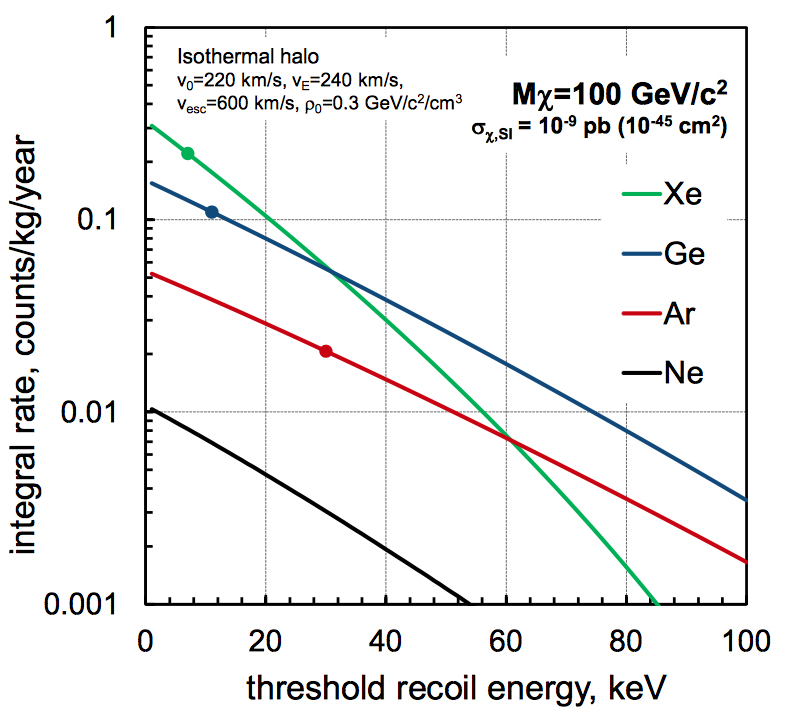
\includegraphics[width=0.6\textwidth]{IntegralRateTargets}
\caption[Expected integral spectra for Xe (green), Ge (blue), Ar (red), and Ne (black) for spin-independent elastic scattering of
$100\ \mathrm{GeV/c^2}$ WIMPs with
cross section $\sigma = 10^{-45}\ \mathrm{cm^{2}}$ per nucleon.]{Expected integral spectra for Xe (green), Ge (blue), Ar (red), and Ne
(black) for spin-independent elastic scattering of $100\ \mathrm{GeV/c^2}$ WIMPs with
cross section $\sigma = 10^{-45}\ \mathrm{cm^{2}}$ per nucleon.  The rates assume perfect energy resolution and are calculated using the
Standard Halo Model.  The dots correspond to average thresholds for each element.  Image credit: \citeref{Cushman2013}.}
\label{fig:material_wimp_rate}
\end{figure}

Liquid noble gas detectors can be single or dual phase.  Dual phase use an electric field to drift electrons to the liquid surface, where
they are extracted across a gas gap and generate a second scintillation.  Single phase detectors measure only the scintillation and are
typically
spherical.  Because they do not drift electrons they benefit from 4$\pi$ photo-detection (in dual phase this would interfere with the
electric field).  Dual phase experiments are discussed in detail in \chapref{chap:liquid_xe}.

Noble liquid experiments that have been or will be built for dark matter searches include the Argon Dark Matter (ArDM) experiment
\citeref{ArDM2013}, DarkSide \citeref{DarkSide2018a, DarkSide2018b, DarkSide2018c}, DarkSide-20k \citeref{DarkSide2018c}, DEAP-3600
\citeref{DEAP2017, DEAP2018}, LUX \citeref{LUX2017a}, LZ \citeref{LZ2018},
PandaX-II \citeref{PandaXII2017}, XMASS \citeref{XMASS2018}, XENON10 \citeref{Angle2008, Aprile2011}, XENON100
\citeref{Aprile2012a, Aprile2016c}, XENON1T \citeref{Aprile2018b}, and XENONnT.  \figref{fig:si_limits} shows the
current status of spin-independent limits before the run combined analysis in \chapref{chap:xenon1t}.

\begin{figure}
\centering
\includegraphics[width=\textwidth]{si_limits}
\caption[Status of spin-independent WIMP cross section from $0.5 \mdash 1000\ \mathrm{GeV/c^2}$ before XENON1T run-combined analysis.]{Status
of spin-independent WIMP cross section from $0.5 \mdash 1000\ \mathrm{GeV/c^2}$ before XENON1T run-combined analysis
(\chapref{chap:xenon1t}).  Regions of possible signals from DAMA/LIBRA (shaded green, \citeref{DAMA2009}) and the silicon
detector of CDMS II (shaded blue, \citeref{CDMS2013}) are shown.  Exclusion limits from PICO-60 (solid yellow line, \citeref{PICO2017}),
DEAP-3600 (dashed purple $> 20\ \mathrm{GeV/c^2}$,
\citeref{DEAP2018}), SuperCDMS (dashed blue, \citeref{SuperCDMS2017}), NEWS-G (dashed purple $< 20\ \mathrm{GeV/c^2}$,
\citeref{NEWSG2018}), CRESST (solid red, \citeref{CRESST2016}), CDMSLite2 (solid blue, \citeref{CDMSLite2016}), LUX
(solid orange, \citeref{LUX2017a}), PandaX-II (solid dark blue 2016
\citeref{PandaXII2016a}, dashed dark blue, 2017 \citeref{PandaXII2017}), XENON100 (solid green, \citeref{Aprile2012c}), and
XENON1T First Results (dashed green, \citeref{Aprile2017f}) are plotted.  Four typical super-symmetric (SUSY) models (CMSSM, NUHM1, NUHM2,
and pMSSM10) with constraints from ATLAS Run
1 are shown (shaded yellow) for reference \citeref{Bagnaschi2015}.  The cross section of neutrino coherent scattering is marked by the
orange dashed
line and shaded region.  Image credit: \citeref{Patrignani2016}.}
\label{fig:si_limits}
\end{figure}


% read https://www.hindawi.com/journals/ahep/2014/387493/ to rewrite above section